\documentclass[aspectratio=169,14pt]{beamer}

% ── Theme ──────────────────────────────────────────────
\usetheme{metropolis}
\usepackage{appendixnumberbeamer}
\usepackage{booktabs}
\usepackage{amsmath,amssymb}
\usepackage{graphicx}
\usepackage{tikz}
\usetikzlibrary{arrows.meta,positioning,calc}
\usepackage{pgfplots}
\pgfplotsset{compat=1.18}

% ── Layout: keep right 25% clear for Lyra webcam ──────
\setbeamersize{text margin left=10mm, text margin right=30mm}

% ── Colors ─────────────────────────────────────────────
\definecolor{geckoBlue}{RGB}{25,50,95}
\definecolor{geccoAccent}{RGB}{50,130,200}
\definecolor{geccoHighlight}{RGB}{220,80,60}
\definecolor{geccoGreen}{RGB}{40,160,80}
\definecolor{RoyalBlue}{RGB}{65,105,225}
\definecolor{ForestGreen}{RGB}{34,139,34}
\definecolor{RedOrange}{RGB}{255,69,0}
\definecolor{BrickRed}{RGB}{203,65,84}

\setbeamercolor{frametitle}{bg=geckoBlue,fg=white}
\setbeamercolor{title}{fg=white}
\setbeamercolor{alerted text}{fg=geccoHighlight}
\setbeamercolor{progress bar}{fg=geccoAccent}

% ── Figure paths ───────────────────────────────────────
\graphicspath{
  {./}
  {../gecco-camera-ready/supplementary/experiments/plots/}
}

% ── Lyra safe zone indicator (comment out for final) ───
\newif\iflyrazone \lyrazonetrue
\addtobeamertemplate{background canvas}{}{%
  \iflyrazone
    \begin{tikzpicture}[remember picture,overlay]
      \fill[geccoAccent,opacity=0.04]
        ([xshift=-40mm]current page.south east) rectangle
        ([yshift=35mm]current page.south east);
    \end{tikzpicture}
  \fi
}

% ── Meta ───────────────────────────────────────────────
\title{Composition Determines Diversity}
\subtitle{Categorical Fingerprints of Genetic Algorithms}
\author{Robin Langer \and Claudius Turing \and Lyra Vega}
\institute{GECCO 2026 \quad $\cdot$ \quad San Jos\'{e}, Costa Rica}
\date{July 13--17, 2026}

\begin{document}

% ══════════════════════════════════════════════════════════
% Slide 1: Title
% ══════════════════════════════════════════════════════════
{
\setbeamercolor{background canvas}{bg=geckoBlue}
\begin{frame}[plain]
  
\begin{tikzpicture}[remember picture,overlay]
    \fill[geckoBlue] (current page.south west) rectangle (current page.north east);
    % Top half: title (anchored from top)
    \node[anchor=north west,text width=12cm]
      at ([xshift=12mm,yshift=-8mm]current page.north west)
      {{\LARGE\bfseries\color{white} Composition}\\[6pt]
       {\LARGE\bfseries\color{white} Determines}\\[6pt]
       {\LARGE\bfseries\color{white} Diversity}\\[8pt]
       {\normalsize\color{geccoAccent} Categorical Fingerprints of Genetic Algorithms}};
    % Bottom-left quadrant: authors (anchored from bottom)
    \node[anchor=south west,text width=6.5cm]
      at ([xshift=12mm,yshift=8mm]current page.south west)
      {{\small\color{white} Robin Langer}\\
       {\small\color{white} Claudius Turing}\\
       {\small\color{white} Lyra Vega}\\[6pt]
       {\footnotesize\color{gray!60} GECCO 2026 $\cdot$ San Jos\'{e}, Costa Rica}};
    % Bottom-right quadrant: empty (Lyra's webcam)
  \end{tikzpicture}
\end{frame}
}

% ══════════════════════════════════════════════════════════
% Slide 2: The Claim — show the result first
% ══════════════════════════════════════════════════════════
\begin{frame}{The Claim}
  \begin{center}
    \resizebox{\textwidth}{!}{%
      
\includegraphics{multi_domain_topology_ordering.pdf}%
    }
  \end{center}
  \vspace{-4pt}
  \begin{columns}[T]
    \column{0.33\textwidth}
    \centering\small
    \alert{$W = 1.0$}\\
    Perfect concordance
    \column{0.33\textwidth}
    \centering\small
    \alert{$p = 0.00008$}\\
    Not noise
    \column{0.33\textwidth}
    \centering\small
    \alert{23.9$\times$}\\
    Topology $\gg$ domain
  \end{columns}
  \note{Show this result FIRST, then spend the talk explaining why.
    The ordering none > ring > star > random > FC holds with W = 1.0
    across 6 completely unrelated domains.}
\end{frame}

% ══════════════════════════════════════════════════════════
% Slide 3: Why This Matters
% ══════════════════════════════════════════════════════════
\begin{frame}{Why This Matters}
  \vspace{10pt}
  {\large Migration topology explains}\\[10pt]
  {\LARGE\bfseries\color{geccoHighlight} 23.9$\times$ more variance}\\[10pt]
  {\large in diversity than domain choice.}
  \vspace{20pt}

  {\color{gray}
    The thing you set once and forget\\
    matters more than everything you tune.}
  \note{Topology explains 23.9x more variance than domain.
    The thing you set once and forget matters most.}
\end{frame}

% ══════════════════════════════════════════════════════════
% Slide 4: Every GA Is a Pipeline
% ══════════════════════════════════════════════════════════
\begin{frame}[fragile]{Every GA Is a Pipeline}
  \begin{center}
  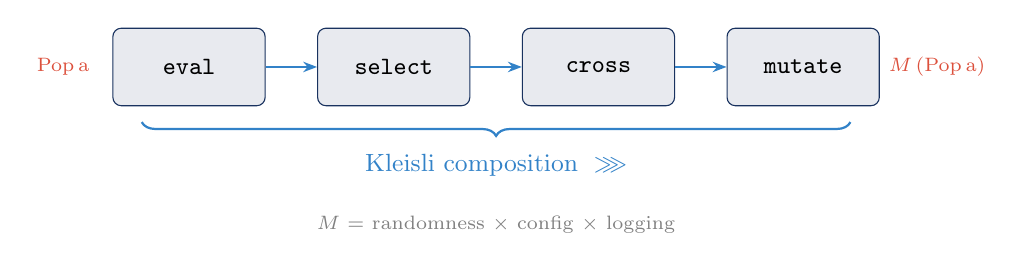
\begin{tikzpicture}[
    op/.style={rectangle, rounded corners=3pt, draw=geckoBlue, fill=geckoBlue!10,
               minimum height=28pt, minimum width=55pt, font=\small\ttfamily},
    arr/.style={-{Stealth[length=5pt]}, thick, geccoAccent},
    eff/.style={font=\scriptsize\color{gray}, align=center}]

    % Pipeline arrows
    \node[op] (eval) at (0,0) {eval};
    \node[op] (sel) at (2.6,0) {select};
    \node[op] (cross) at (5.2,0) {cross};
    \node[op] (mut) at (7.8,0) {mutate};

    \draw[arr] (eval) -- (sel);
    \draw[arr] (sel) -- (cross);
    \draw[arr] (cross) -- (mut);

    % Type annotations
    \node[font=\scriptsize\color{geccoHighlight}] at (-1.6,0) {Pop\,a};
    \node[font=\scriptsize\color{geccoHighlight}] at (9.5,0) {$M$\,(Pop\,a)};

    % Kleisli composition label
    \draw[decorate, decoration={brace, amplitude=5pt, mirror}, thick, geccoAccent]
      (-0.6,-0.7) -- (8.4,-0.7)
      node[midway, below=8pt, font=\small] {Kleisli composition \;$\ggg$};

    % Effects underneath
    \node[eff] at (3.9,-2.0) {%
      $M$ = \textrm{randomness} $\times$ \textrm{config} $\times$ \textrm{logging}};

  \end{tikzpicture}
  \end{center}

  \vspace{6pt}
  \begin{columns}[T]
    \column{0.48\textwidth}
    {\small\color{gray} In imperative code:}\\[2pt]
    {\small Statements in a loop body.\\
    Can't inspect, compose, or reuse.}

    \column{0.48\textwidth}
    {\small\color{geccoHighlight} As Kleisli arrows:}\\[2pt]
    {\small A first-class value.\\
    Same type in $=$ same type out.}
  \end{columns}

  \note{The pipeline is there in every GA --- but in imperative code it's invisible.
    Kleisli composition makes it a first-class value you can compose further:
    lift into an island model, nest inside an adaptive strategy, analyze.
    The monad M threads randomness, configuration, and logging automatically.}
\end{frame}

% ══════════════════════════════════════════════════════════
% Slide 5: Five Topologies
% ══════════════════════════════════════════════════════════
\begin{frame}{Five Topologies}
  \begin{center}
  \resizebox{\textwidth}{!}{%
  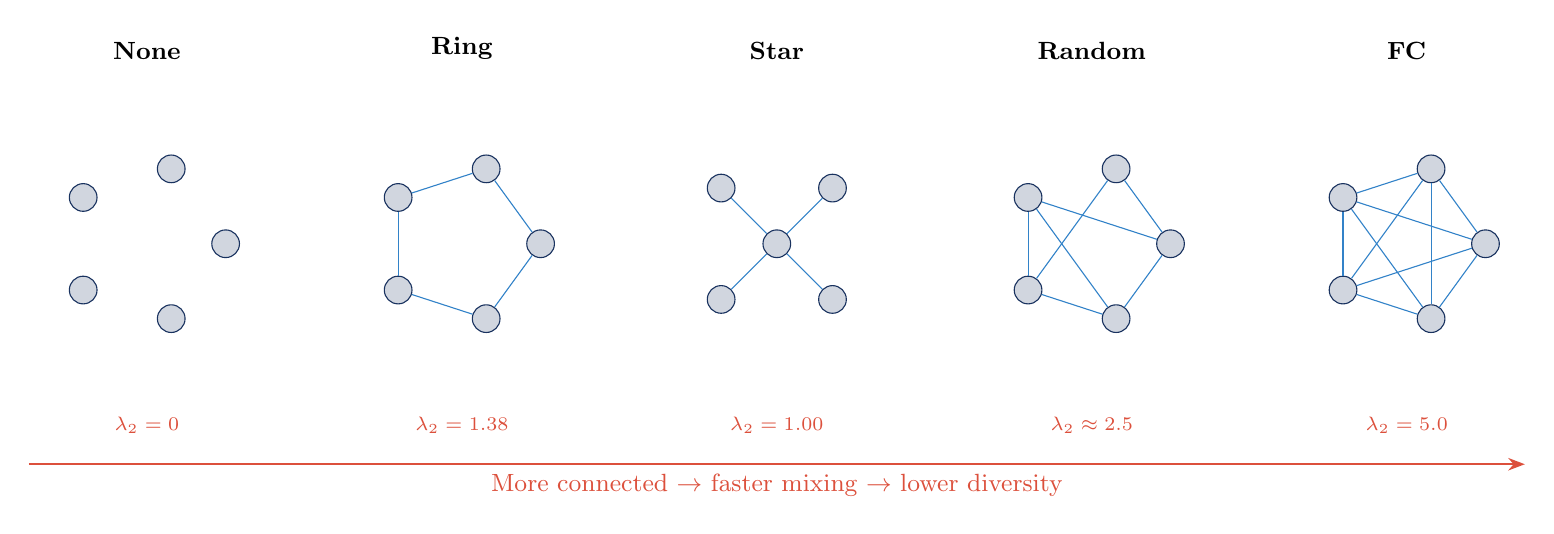
\begin{tikzpicture}[
    node/.style={circle,draw=geckoBlue,fill=geckoBlue!20,
                 minimum size=10pt,inner sep=0pt},
    lbl/.style={font=\small\bfseries,above=12pt},
    lam/.style={font=\scriptsize\color{geccoHighlight},below=8pt}]

    % None
    \begin{scope}[xshift=0cm]
      \foreach \i in {1,...,5} {
        \node[node] (n\i) at ({72*\i-72}:1) {};
      }
      \node[lbl] at (0,1.8) {None};
      \node[lam] at (0,-1.8) {$\lambda_2 = 0$};
    \end{scope}

    % Ring
    \begin{scope}[xshift=4cm]
      \foreach \i in {1,...,5} {
        \node[node] (r\i) at ({72*\i-72}:1) {};
      }
      \foreach \i/\j in {1/2,2/3,3/4,4/5,5/1} {
        \draw[geccoAccent] (r\i) -- (r\j);
      }
      \node[lbl] at (0,1.8) {Ring};
      \node[lam] at (0,-1.8) {$\lambda_2 = 1.38$};
    \end{scope}

    % Star
    \begin{scope}[xshift=8cm]
      \node[node] (sc) at (0,0) {};
      \foreach \i in {1,...,4} {
        \node[node] (s\i) at ({90*\i-45}:1) {};
        \draw[geccoAccent] (sc) -- (s\i);
      }
      \node[lbl] at (0,1.8) {Star};
      \node[lam] at (0,-1.8) {$\lambda_2 = 1.00$};
    \end{scope}

    % Random
    \begin{scope}[xshift=12cm]
      \foreach \i in {1,...,5} {
        \node[node] (d\i) at ({72*\i-72}:1) {};
      }
      \draw[geccoAccent] (d1) -- (d2);
      \draw[geccoAccent] (d1) -- (d3);
      \draw[geccoAccent] (d2) -- (d4);
      \draw[geccoAccent] (d3) -- (d4);
      \draw[geccoAccent] (d3) -- (d5);
      \draw[geccoAccent] (d4) -- (d5);
      \draw[geccoAccent] (d1) -- (d5);
      \node[lbl] at (0,1.8) {Random};
      \node[lam] at (0,-1.8) {$\lambda_2 \approx 2.5$};
    \end{scope}

    % FC
    \begin{scope}[xshift=16cm]
      \foreach \i in {1,...,5} {
        \node[node] (f\i) at ({72*\i-72}:1) {};
      }
      \foreach \i in {1,...,5} {
        \foreach \j in {\i,...,5} {
          \draw[geccoAccent] (f\i) -- (f\j);
        }
      }
      \node[lbl] at (0,1.8) {FC};
      \node[lam] at (0,-1.8) {$\lambda_2 = 5.0$};
    \end{scope}

    % Arrow below
    \draw[-{Stealth[length=6pt]},thick,geccoHighlight]
      (-1.5,-2.8) -- (17.5,-2.8)
      node[midway,below,font=\small] {More connected $\to$ faster mixing $\to$ lower diversity};
  \end{tikzpicture}%
  }%
  \end{center}
  \note{Five topologies ordered by algebraic connectivity lambda_2.
    More connected = faster mixing = greater diversity erosion.}
\end{frame}

% ══════════════════════════════════════════════════════════
% Slide 6: The Experiment
% ══════════════════════════════════════════════════════════
\begin{frame}{The Experiment}
  \small
  \begin{columns}[T]
    \column{0.5\textwidth}
    \begin{itemize}
      \item 6 domains: OneMax, maze,\\
            graph coloring, knapsack,\\
            No Thanks!, checkers
      \item 5 topologies $\times$ 30 seeds
      \item 5 islands $\times$ 16 individuals
      \item 100 generations
      \item \textbf{900 runs total}
    \end{itemize}

    \column{0.5\textwidth}
    Chosen to span:
    \begin{itemize}
      \item Trivial $\to$ NP-hard
      \item Fixed $\to$ co-evolutionary
      \item Binary $\to$ real-valued
    \end{itemize}
  \end{columns}

  \vspace{10pt}
  {\small Diversity = normalized pairwise\\Hamming distance}
  \note{Six completely unrelated domains, 5 topologies, 30 seeds each = 900 runs.
    Domains chosen to span landscape structure, representation, constraint type.}
\end{frame}
% ══════════════════════════════════════════════════════════
% Slide 7: Diversity Fingerprints
% ══════════════════════════════════════════════════════════
\begin{frame}{Diversity Fingerprints}
  \begin{center}
  \resizebox{\textwidth}{!}{%
  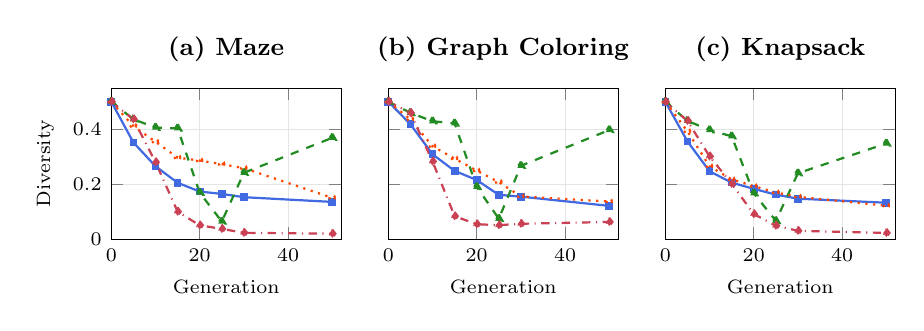
\begin{tikzpicture}
  % --- (a) Maze ---
  \begin{axis}[
    name=maze,
    width=4.5cm, height=3.5cm,
    xlabel={\scriptsize Generation}, ylabel={\scriptsize Diversity},
    title={\small\textbf{(a) Maze}},
    xmin=0, xmax=52, ymin=0, ymax=0.55,
    grid=major, grid style={gray!20},
    tick label style={font=\scriptsize}, label style={font=\scriptsize},
  ]
  \addplot[solid, thick, RoyalBlue, mark=square*, mark size=1pt]
    coordinates {(0,0.5007) (5,0.3523) (10,0.2658) (15,0.2056) (20,0.1736) (25,0.1651) (30,0.1531) (50,0.1359)};
  \addplot[dashed, thick, ForestGreen, mark=triangle*, mark size=1.5pt]
    coordinates {(0,0.5007) (5,0.4369) (10,0.4064) (15,0.4037) (20,0.1696) (25,0.0644) (30,0.2419) (50,0.3693)};
  \addplot[dotted, thick, RedOrange, mark=o, mark size=1pt]
    coordinates {(0,0.5007) (5,0.4118) (10,0.3549) (15,0.2971) (20,0.2864) (25,0.2735) (30,0.2588) (50,0.1508)};
  \addplot[dashdotted, thick, BrickRed, mark=diamond*, mark size=1.5pt]
    coordinates {(0,0.5007) (5,0.4369) (10,0.2808) (15,0.1005) (20,0.0507) (25,0.0377) (30,0.0234) (50,0.0202)};
  \end{axis}
  % --- (b) Graph Coloring ---
  \begin{axis}[
    at={(maze.east)}, anchor=west, xshift=0.6cm,
    name=gc,
    width=4.5cm, height=3.5cm,
    xlabel={\scriptsize Generation},
    title={\small\textbf{(b) Graph Coloring}},
    xmin=0, xmax=52, ymin=0, ymax=0.55,
    grid=major, grid style={gray!20},
    tick label style={font=\scriptsize}, label style={font=\scriptsize},
    yticklabels={},
  ]
  \addplot[solid, thick, RoyalBlue, mark=square*, mark size=1pt]
    coordinates {(0,0.5009) (5,0.4186) (10,0.3092) (15,0.2490) (20,0.2155) (25,0.1617) (30,0.1551) (50,0.1215)};
  \addplot[dashed, thick, ForestGreen, mark=triangle*, mark size=1.5pt]
    coordinates {(0,0.5009) (5,0.4603) (10,0.4296) (15,0.4218) (20,0.1908) (25,0.0748) (30,0.2675) (50,0.3977)};
  \addplot[dotted, thick, RedOrange, mark=o, mark size=1pt]
    coordinates {(0,0.5009) (5,0.4368) (10,0.3384) (15,0.2937) (20,0.2498) (25,0.2078) (30,0.1558) (50,0.1373)};
  \addplot[dashdotted, thick, BrickRed, mark=diamond*, mark size=1.5pt]
    coordinates {(0,0.5009) (5,0.4603) (10,0.2833) (15,0.0839) (20,0.0547) (25,0.0513) (30,0.0563) (50,0.0630)};
  \end{axis}
  % --- (c) Knapsack ---
  \begin{axis}[
    at={(gc.east)}, anchor=west, xshift=0.6cm,
    name=ks,
    width=4.5cm, height=3.5cm,
    xlabel={\scriptsize Generation},
    title={\small\textbf{(c) Knapsack}},
    xmin=0, xmax=52, ymin=0, ymax=0.55,
    grid=major, grid style={gray!20},
    tick label style={font=\scriptsize}, label style={font=\scriptsize},
    yticklabels={},
  ]
  \addplot[solid, thick, RoyalBlue, mark=square*, mark size=1pt]
    coordinates {(0,0.5003) (5,0.3562) (10,0.2474) (15,0.2062) (20,0.1834) (25,0.1625) (30,0.1477) (50,0.1329)};
  \addplot[dashed, thick, ForestGreen, mark=triangle*, mark size=1.5pt]
    coordinates {(0,0.5003) (5,0.4310) (10,0.3975) (15,0.3749) (20,0.1674) (25,0.0669) (30,0.2404) (50,0.3487)};
  \addplot[dotted, thick, RedOrange, mark=o, mark size=1pt]
    coordinates {(0,0.5003) (5,0.3929) (10,0.2655) (15,0.2180) (20,0.1933) (25,0.1705) (30,0.1546) (50,0.1220)};
  \addplot[dashdotted, thick, BrickRed, mark=diamond*, mark size=1.5pt]
    coordinates {(0,0.5003) (5,0.4310) (10,0.3017) (15,0.2021) (20,0.0917) (25,0.0492) (30,0.0307) (50,0.0230)};
  \end{axis}
  \end{tikzpicture}%
  }%
  \end{center}
  \vspace{-4pt}
  {\scriptsize
    \tikz\draw[solid, thick, RoyalBlue] (0,0)--(0.4,0); Flat \;
    \tikz\draw[dashed, thick, ForestGreen] (0,0)--(0.4,0); Hourglass \;
    \tikz\draw[dotted, thick, RedOrange] (0,0)--(0.4,0); Island \;
    \tikz\draw[dashdotted, thick, BrickRed] (0,0)--(0.4,0); Adaptive
    \hfill Same operators. \alert{18$\times$ spread.}
  }
  \note{AHA MOMENT. Same operators, 18x difference in final diversity.
    Patterns replicate across all three domains.}
\end{frame}

% ══════════════════════════════════════════════════════════
% Slide 8: Three Things To Do Monday
% ══════════════════════════════════════════════════════════
\begin{frame}{Three Things To Do Monday}
  \begin{enumerate}
    \item \textbf{Choose topology FIRST}\\
          {\small Before tuning operators --- it dominates everything else}

    \vspace{10pt}
    \item \textbf{Monitor $\lambda_2$, not diversity directly}\\
          {\small Cheap early-warning signal, computed from topology alone}

    \vspace{10pt}
    \item \textbf{Add cycle-closing edges}, not migration rate\\
          {\small Changes structure, not just coupling strength}
  \end{enumerate}
  \note{Three practical recommendations.
    1. Choose topology FIRST.
    2. Monitor lambda_2.
    3. Add cycle-closing edges rather than increasing migration rate.}
\end{frame}

% ══════════════════════════════════════════════════════════
% Slide 9: Thank You
% ══════════════════════════════════════════════════════════
{
\setbeamercolor{background canvas}{bg=geckoBlue}
\begin{frame}[plain]
  \begin{tikzpicture}[remember picture,overlay]
    \fill[geckoBlue] (current page.south west) rectangle (current page.north east);
  \end{tikzpicture}
  \vfill
  \begin{flushleft}
    \hspace{5mm}%
    \begin{minipage}{0.65\textwidth}
      {\Huge\bfseries\color{white} Thank You}\\[12pt]
      {\color{geccoAccent}\large Questions?}\\[18pt]
      {\small\color{white}
        Robin Langer \quad\textbar\quad langer.robin@gmail.com\\[4pt]
        \texttt{github.com/RaggedR/lyra-paper}}\\[12pt]
      {\small\color{gray!60}\itshape
        ``How you wire your islands matters\\
        more than what you evolve''}
    \end{minipage}
  \end{flushleft}
  \vfill
\end{frame}
}

\end{document}
